% ==================================================================
% 4.4 So sanh voi detector nhe (MOT giao thuc duy nhat)
% file: sections/11_exp_baselines.tex
% So lieu: runs/paper_queue/UNIFIED.json (accuracy + mCP + retain)
%          runs/paper_queue/BASELINES_TABLE.md (params / GFLOPs)
% ==================================================================
\subsection{Comparison with Lightweight Detectors}
\label{sec:baselines}

Table~\ref{tab:baselines} compares five detectors spanning three paradigms against
ours. Every row, including the corrupted columns, came from the single evaluation
path of Section~\ref{sec:setup}. We report it in full rather than selectively, and
the two accuracy columns disagree about who wins.

\begin{table}[t]
\centering
\caption{VisDrone person subset, every row measured by the same evaluation code
(Section~\ref{sec:setup}). $\mathrm{mCP}$ is mean AP$_{50:95}$ over the three
vibration levels, that is, accuracy \emph{in flight}; retention is
$\mathrm{mCP}/\mathrm{AP}_{\mathrm{clean}}$, mean $\pm$ std over three seeds. YOLO
and RT-DETR rows start from COCO-pretrained weights while SteadyDet rows train from
scratch, which favours the baselines. \emph{The clean and the mCP columns rank the
table differently, and mCP is the one the aircraft experiences.}}
\label{tab:baselines}
\setlength{\tabcolsep}{4.5pt}
\begin{tabular}{lcccccc}
\toprule
Model & Params (M) & GFLOPs & AP$_{50}$ & AP$_{50:95}$ & mCP & retain\% \\
\midrule
RT-DETR-l                   & 32.81 & 108.0 & 0.5909 & 0.2502$^\dagger$ & 0.0641 & \ms{25.6}{1.1} \\
YOLOv10-n                   & 2.71 & 8.4 & 0.6043 & 0.2730 & 0.0538 & \ms{19.7}{1.4} \\
YOLOv8-n                    & 3.01 & 8.2 & 0.6033 & 0.2684 & 0.0522 & \ms{19.5}{.8} \\
YOLO26-n                    & 2.50 & 5.8 & 0.5898 & 0.2675 & 0.0507 & \ms{19.0}{1.0} \\
YOLO11-n                    & 2.59 & 6.4 & \best{0.6119} & \best{0.2768} & 0.0557 & \ms{20.1}{1.2} \\
\quad + vib.-aware          & 2.59 & 6.4 & 0.6057 & 0.2700 & 0.0542 & \ms{20.1}{1.3} \\
\midrule
SteadyDet-W                  & 1.00 & 12.9 & 0.5800 & 0.2349 & 0.0521 & \ms{22.2}{.9} \\
\quad \textbf{+ vib.-aware} & 1.00 & 12.9 & 0.5511 & 0.2219 & \best{0.0874} & \best{\ms{39.4}{.3}} \\
SteadyDet-N                  & \textbf{1.17} & \textbf{4.6} & 0.5127 & 0.1892 & 0.0318 & \ms{16.8}{.7} \\
\quad + consistency         & 1.17 & 4.6 & 0.4837 & 0.1746 & 0.0524 & \ms{30.0}{.6} \\
\quad \textbf{+ vib.-aware} & \textbf{1.17} & \textbf{4.6} & 0.4731 & 0.1708 & 0.0617 & \ms{36.2}{.7} \\
\bottomrule
\multicolumn{7}{l}{\footnotesize $^\dagger$ RT-DETR's reference implementation
scale-fills rather than letterboxes its input; under our}\\
\multicolumn{7}{l}{\footnotesize \phantom{$^\dagger$} common pipeline its clean AP
is depressed. Native harness: $0.3340$. mCP and retention are ratios}\\
\multicolumn{7}{l}{\footnotesize \phantom{$^\dagger$} within that same pipeline and
are unaffected.}\\
\end{tabular}
\end{table}

\subsubsection{On clean data our architecture does not lead its class.}
Every YOLO nano variant exceeds it, and we do not explain that away. COCO
pretraining is one factor and our from-scratch training a second, but the gap is
larger than those plausibly account for, and efficiency does not close it: $4.6$
GFLOPs against $5.8$ for the closest baseline is a $21\%$ saving that does not pay
for the accuracy difference. On the benchmark, we lose.

\subsubsection{Under vibration the ranking reverses, and that is the condition that matters.}
The mCP column orders the table almost opposite to the clean column. SteadyDet-N
with vibration-aware training reaches $0.0617$ against $0.0557$ for the strongest
baseline, at $45\%$ of its parameters and $72\%$ of its compute. RT-DETR-l leads it
on the mCP average ($0.0641$), but not where it counts: at sev2, the severity of an
airframe in ordinary forward flight, RT-DETR reaches $0.0389 \pm 0.0014$ against our
$0.0518 \pm 0.0019$, a gap of five pooled standard deviations from a network with
$28\times$ the parameters and $23\times$ the compute. At sev3 the two are within
noise ($0.0100 \pm 0.0017$ against $0.0111 \pm 0.0002$) and we claim no ordering
there. The margin over YOLO11-n at sev2 is a factor of $2.5$.

SteadyDet-W leads the whole table at $0.0874$, on fewer parameters than SteadyDet-N
but $2.8\times$ the compute, and we say plainly that it is the more accurate of our
two networks under vibration. SteadyDet-N is the primary model because compute, not
parameter count, is what binds on the target platform: a following system must fit
detection, tracking and control into one frame budget, and $12.9$ GFLOPs does not
leave room for the rest. Per unit of compute the ordering is unambiguous, with
SteadyDet-N returning $0.0134$ mCP per GFLOP against $0.0087$ for the best baseline
and $0.0068$ for SteadyDet-W.

A reader should object that we compare our treated models against untreated
baselines, and that objection is why Section~\ref{sec:generality} matters here. We
applied the identical regime to YOLO11-n and it does not respond: treated, it
reaches mCP $0.0542$, marginally \emph{below} its untreated $0.0557$. The
comparison is therefore between each detector at its own best, not against a
handicapped one. We tested only YOLO11-n this way, so for the other three baselines
the objection stands unanswered, and we say so rather than assume the null
generalises.

The claim is accordingly narrow and, we think, the useful one: for a vibrating
airframe with a few GFLOPs of budget, the detector to choose is not the one that
wins the benchmark, but a smaller one whose training distribution contains the
corruption. Our untreated baseline is the worst row in the table at $0.0318$, so
neither half of that sentence can be dropped.

\subsubsection{Robustness is not a by-product of accuracy.}

\begin{figure}[t]
\centering
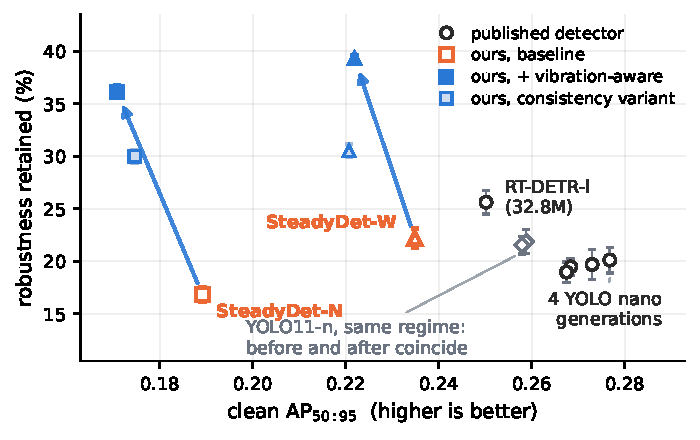
\includegraphics[width=0.95\textwidth]{figures/fig4_tradeoff.pdf}
\caption{Clean accuracy against robustness retained, one point per model, error bars
over three seeds. The published detectors occupy the lower right: more accuracy, no
more robustness, with four YOLO generations landing within a point of each other. The
arrows are the effect of vibration-aware training; the pale markers are the
consistency variant, which lands short of it. The two grey diamonds are YOLO11-n
before and after the identical regime, and they sit on top of one another.}
\label{fig:tradeoff}
\end{figure}

Fig.~\ref{fig:tradeoff} plots clean accuracy against retention. Hendrycks and
Dietterich already reported, for ImageNet classifiers, that robustness measured
relative to clean accuracy barely improved across a decade of architectural
progress~\cite{hendrycks2019benchmarking}; we find the same decoupling holds for
compact aerial detectors under a corruption they were never designed for, which is
worth stating because the detectors here span four years and three paradigms. Four
YOLO generations sit within a point of one another at $19$ to $20\%$ despite their
differences, and the transformer reaches $25.6 \pm 1.1\%$ only by spending
$28\times$ our parameters. Robustness therefore has to be measured and optimised
separately rather than expected to follow from clean accuracy. The arrows show the
alternative: a large robustness gain for a small loss of clean accuracy, obtained by
changing the training distribution rather than the network.

Our re-measured clean figures sit slightly below the detectors' own harnesses
($0.2684$ against $0.2787$ for YOLOv8-n) because each applies different confidence,
detection-count and area conventions, by margins comparable to the gaps between the
baselines themselves. That is why harnesses cannot be mixed within one table.
